\chapter{Modelli e formulazioni matematiche}

\section{The Traveling Salesman Problem}
Il Traveling Salesman Problem (TSP) è il problema più noto dell'ottimizzazione combinatoria.
Siano date $n$ città e i costi $c_{ij}$ per andare dalla città $i$ alla città $j$.
Si vuole determinare un cammino che parte da una città (diciamo $i_{1}$), visitare una ed una sola volta tutte le rimanenti città e terminare nella città di partenza $i_{1}$.
Inoltre si vuole che il costo di tale cammino sia minimo.\newline
Ha molteplici applicazioni pratiche e teoriche perche è la struttura di molti problemi pratici.\newline
Si è soliti modella il TSP come segue:
\begin{itemize}
	\item è dato un grafo orientato (o non orientato) $G = (N,A)$
	dove $N$ è un insieme di $n$ vertici e $A$ è un insieme di $m$ archi.
	
	Ad ogni arco $\emph{(i,j)} \in \emph{A}$ è associato un costo $c_{ij}$.
	
	Un circuito hamiltoniano di $G$ è un circuito che passa per ogni vertice una ed una sola volta.\newline
	Il costo di un circuito hamiltoniano di $G$ è pari alla somma dei costi degli archi che compongono il circuito;
	\item il problema del TSP è di trovare un grafo $G$, con una data matrice dei costi [$c_{ij}$], un circuito hamiltoniano di costo minimo.
\end{itemize}
\newpage
\subsection{Formulazioni Matematiche del TSP}
In letteratura esistono molteplici (e a volte fantasiose) formulazioni del TSP.\newline
Presentiamo le due formulazioni più note e su cui si basano i metodi esatti più efficienti.

\subsubsection{TSP asimmetrico}
I costi $c_{ij}$ non verificano $c_{ij} = c_{ji}\;\forall\;i,j$ con $i < j$.\newline
Sia $x_{ij}$ una variabile $(0-1)$ associata ad ogni arco $(i,j) \in A$ dove $x_{ij}=1$ se l'arco $(i,j)$ è nella soluzione ottima e $x_{ij}=0$ altrimenti.\newline

\begin{equation}
	Min\;\;\displaystyle\sum_{i\in N}^{} \sum_{j\in N}^{} c_{ij} x_{ij}
\end{equation}
\begin{equation}
	s.t.\;\;\displaystyle\sum_{i\in N}^{} x_{ij} = 1,\;\;\forall j \in N
\end{equation}
\begin{equation}
	\;\;\;\;\;\;\;\displaystyle\sum_{j\in N}^{} x_{ij} = 1,\;\;\forall i \in N
\end{equation}
\begin{equation}
	\;\;\;\;\;\;\;\;\;\;\;\;\;\;\;\;\;\;\displaystyle\sum_{i\in S}^{} \sum_{j\in N\setminus S}^{} x_{ij} \ge 1,\;\;\forall S \subset N
\end{equation}
\begin{equation}
	\;\;\;\;\;\;\;\;\;\;x_{ij} \in \{0,1\}\;,\;\forall (i,j) \in A
\end{equation}

Il vincolo $1.4$ impone che ogni soluzione ammissibile debba contenere almeno un arco $(i,j)$ con $i\in S$ e $j\in N\setminus S$ per ogni sottoinsieme $S$ di $N$.
Un'alternativa al vincolo $1.4$ è:
\begin{equation}\tag{1.4'}
\;\;\;\;\;\;\;\;\;\;\;\;\;\;\;\;\;\;\displaystyle\sum_{i\in S}^{} \sum_{j\in S}^{} x_{ij} \le |S| - 1,\;\;\forall S \subset N
\end{equation}

\subsubsection{TSP simmetrico}
Sia dato un grafo non-orientato $G=(N,A)$ con $c_{ij} = c_{ji}\:,\forall i,j\in N$.\newline
Gli archi di $A$ sono numerati da $1$ a $m$. L'arco di indice $l$ corrisponde a $(\alpha_{l},\beta_{l})$ con $\alpha_{l} < \beta_{l}$.\newline
$A_{i}$ è il sottoinsieme degli indici degli archi che incidono sul vertice $i$:
\begin{center}
	$A_{i} = \{l:\;l=1,m\;\;s.t.\;\alpha_{l}=i\;or\;\beta_{l}=i\}$
\end{center}

Per una dato $S\in N$ e $\bar{S} = N\setminus S$ indichiamo con $(S, \bar{S})$ il sottoinsieme degli indici degli archi per cui $\alpha_{l}\in S$ e $\beta_{l}\in \bar{S}$ oppure $\alpha_{l}\in \bar{S}$ e $\beta_{l}\in S$.

Ad ogni arco di incide $l$ è associato un costo $d_{l}=c_{\alpha_{l}\beta_{l}}$ e $x_{l}\in \{0,1\}$ è una variabile che vale 1 se e solo se l'arco di indice $l$ è nella soluzione ottima.
\begin{equation}
	Min\;\;\displaystyle\sum_{l=1}^{} d_{l}\:x_{l}
\end{equation}
\begin{equation}
	s.t.\;\;\displaystyle\sum_{l\in A_{i}}^{} x_{l}=2,\; \forall i\in N
\end{equation}
\begin{equation}
	\;\;\;\;\;\;\;\;\;\displaystyle\sum_{l\in (S, \bar{S})}^{} x_{l} \ge 1,\;\forall S \subset N
\end{equation}
\begin{equation}
	x_{l}\in \{0,1\},\;\;l=1,...,m
\end{equation}

\subsection{Eliminazione subtours di Miller, Tucker, Zemlin (1960)}
Sia $u_{i}$ una variabile intera il cui valore sappresenta la posizione che il vertice $i$ occupa nel tour.

\begin{center}
	Es. tour (1,4,5,3,2,1) per TSP con n=5 vertici, si ha $u_{1}=1,\;u_{2}=5,\;u_{3}=4,\;u_{4}=2,\;u_{5}=3$	
\end{center}

Miller, Tucker e Zemlin propongono in alternativa a:
\begin{equation}\tag{*}
	\displaystyle\sum_{i\in S}^{}\sum_{j\in N\setminus S}^{} x_{ij} \ge 1,\;\;\forall S\subset N
\end{equation}
hanno imposto i seguenti vincoli:
\begin{equation}
	u_{i}-u_{j}+nx_{ij}\le n-1,\;\; i=1,...,n\:,\;j=2,...,n
\end{equation}
Ogni tour hamiltoniano soddisfa questi vincoli e ogni subtour li viola.\newline
\begin{wrapfigure}[5]{l}{0.5\textwidth}
	\vspace{-2em}
	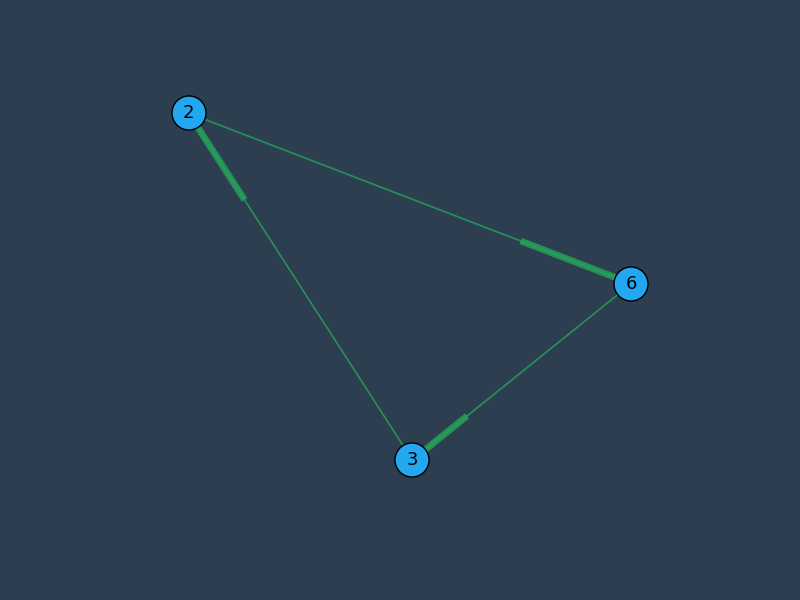
\includegraphics[height=5cm]{images/graph1.png}
	\caption{Grafo orientato}
\end{wrapfigure}
\begin{description}
	\vspace{1.5em}
	\item $u_{2}-u_{6}+n\;\cdot x_{2,6}\le n-1$
	\item $u_{6}-u_{3}+n\;\cdot x_{6,3}\le n-1$
	\item $u_{3}-u_{2}+n\;\cdot x_{3,2}\le n-1$
	\item {\hskip 5.6em}$\downarrow$
	\item {\hskip 3em}$3n \le 3(n-1)$
\end{description}\newpage

\subsection{Il Traveling salesman problem con time windows (TSPTW)}
È una variante del TSP che ha molte applicazioni.

Sia dato un grafo orientato $G=(V,A)$ di $n+1$ vertici $(V=\{0,1,...,n\})$.

Ad ogni arco $(i,j)\in A$ sono associati
\begin{itemize}
	\item un costo $c_{ij} \ge 0$
	\item un tempo di percorrenza $\theta_{ij}\ge 0$
\end{itemize}
Ad ogni vertice è associato un intervallo $[r_{i},d_{i}]$ chiamato "time window" che rappresenta l'orario in cui il vertice $i$ può essere vistato dal "salesman".

Ovvero il salesman può visitare $i$ ad ogni tempo $t\in \mathbb{Z}^{+}$ con $r_{i}\le t\le d_{i}$.\newline
Il problema consiste nel trovare una sequenza dei vertici di $G$ che parte dal vertice $0$ al tempo $0$ e finisce al nodo $0$ tale che sia il minimo il costo del circuito e il tempo di arrivo al nodo $i$ sia nell'intervallo $[r_{i},d_{j}],\;\forall i\in V$.\newline
Si consideri la sequenza $(0,i,..,i_{k-1},i_{k},...,i_{n},0)$ e sia $t_{i_{k}}$ il tempo di arrivo al vertice $i_{k},\; k=0,1,...,n+1$.

I tempi di arrivo sono calcolati come:
\begin{equation}
	t_{0}=0
\end{equation}
\begin{equation}
	t_{i_{k}}=\max \{t_{i_{k-1}}+\theta_{i_{k-1}}\cdot i_{k},\; r_{i_{k}}\}
\end{equation}

\subsubsection{Formulazione del TSPTW}
Sia $x_{ij}$ una variabile binaria intera che assume il valore $1$ se il vertice $i$ è visitato immediatamente prima di $i$ e $x_{ij}=0$ altrimenti.
\begin{flalign}
	& Min\;\;\displaystyle\sum_{(i,j)\in A}^{}c_{ik}x_{ij} \\
	& s.t.\;\;\;\;\displaystyle\sum_{i\in A_{j}^{-}}^{}x_{ij}=1,\;\;\forall j\in V \\		
	& \;\;\;\;\;\;\;\;\displaystyle\sum_{j\in A_{i}^{+}}^{}x_{ij}=1,\;\;\forall i\in V \\
	& \;\;\;\;\;\;\;\;t_{i}+\theta_{ij}-t_{j}\le M(1-x_{ij},\;\;\forall (i,j)\in A,\; j\ne 0) \\
	& \;\;\;\;\;\;\;\;t_{i}\le d_{i},\;\;\forall i\in V \\
	& \;\;\;\;\;\;\;\;t_{i}\ge r_{i},\;\;\forall i\in V \\
	& \;\;\;\;\;\;\;\;x_{ij}\in \{0,1\},\;\;\forall \in A \\
	& \;\;\;\;\;\;\;\;t_{i}\in \mathbb{N}^{+},\;\;\forall i\in V
\end{flalign}

dove 
\begin{flalign*}
	& A_{i}^{+}=\{j\in V:(i,j)\in A\} \\
	& A_{i}^{-}=\{j\in V:(i,j)\in A\} \\
	& M\;è\;un\;intero\;grande\;a\;piacere \\
	& r_{0}=d_{0}=0
\end{flalign*}
\newpage

\section{Project scheduling with resource constraints (PSR)}
\`E dato un insieme $\mathbb{X}=\{1,...,n\}$ di $n$ jobs.

Sono disponibili $m$ risorse dove ogni risorsa $k$ ha una disponibilità $b_{k}$ ad ogni istante del periodo di scheduling.

Ogni job $i$ ha un tempo di processo $d_{i}$ e la sua esecuzione, una volta iniziata, non può essere interrotta.

Il job $i$ per essere eseguito richiede $b_{ik}$ unità della risorsa $k$ per ciascun intervallo di tempo in cui rimane in esecuzione.\newline
\`E dato un grafo $G=(X,H)$ di precedenze, dove ogni arco $(i,j)\in H$ impone che il job $j$ può iniziare solo dopo che il job $i$ è stato completato.

\begin{itemize}
	\item Si vuole determinare il tempo di inizio di processo di ogni job in modo che siano soddisfatti i vincoli di precedenza, i vincoli sulle risorse e sia minima la durata complessiva del progetto
\end{itemize}

\subsection{Esempio di PSR}
Siano dati $n=11$ jobs e $m=3$ risorse con $b_{1}=b_{2}=b_{3}=4$ e un grafo $H$ delle precedenze corrispondenti agli archi della figura ~\ref{fig:grafoHDellePrecedenze}.

Si osservi che i jobs $2$ e $3$ non possono essere eseguiti in parallelo poiché $r_{2,1}+r_{3,1}=5 > b_{1}$!

\begin{figure}[h]
	\caption{Grafo H delle precedenze}
	\centering
	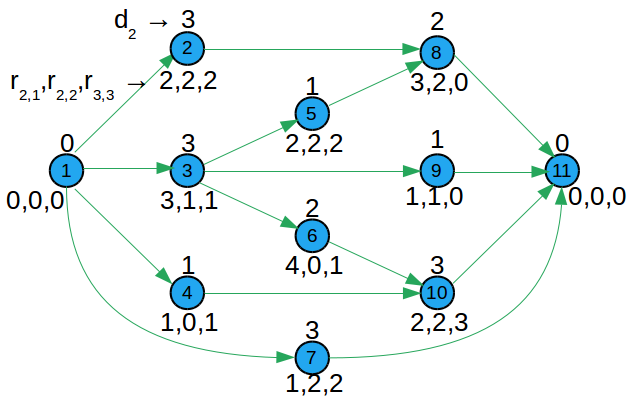
\includegraphics[height=6.5cm]{images/graph2.png}
	\label{fig:grafoHDellePrecedenze}
\end{figure}

\subsection{Formulazione del PSR}
Sia $\xi_{it}$ una variabile binaria 0-1 che vale 1 se e solo se il job $i$ viene messo in esecuzione al tempo $t$.

Sia $T_{max}$ un upper bound sulla durata del progetto.

\begin{flalign}
	& Min \displaystyle\sum_{t=1}^{T_{max}}t\;\xi_{n t} \\
	& \;\;s.t. \displaystyle\sum_{t=1}^{T_{max}}t\;\xi_{i t} = 1,\;\;\;i=1,...,n \\
	& \;\;\;\;\;\;\;\displaystyle\sum_{t=1}^{T_{max}}t\;\xi_{j t} - \displaystyle\sum_{t=1}^{T_{max}}t\;\xi_{i t} \ge d_{i},\;\;\;\forall (i,j)\in H \\
	& \;\;\;\;\;\;\;\displaystyle\sum_{i=1}^{n}r_{ik}\displaystyle\sum_{\tau=t-d_{i}+1}^{t}\xi_{i\tau}\le b_{k},\;\;\;t=1,...,T_{max}\;e\;k=1,...,m \\
	& \;\;\;\;\;\;\;\;\;\;\;\;\;\;\;\;\;\;\;\;\;\;\;\;\;\;
	\;\;\;\;\;\;\xi_{it}\in\{0,1\},\;\;\; i=1,...,n\;e\;t=1,...,T_{max}
\end{flalign}
Si osservi che:
\begin{flalign*}
	& \displaystyle\sum_{\tau=t-d_{i}+1}^{t}\xi_{i \tau}=1\;\;\;se\;il\;job\;i\;è\;in\;esecuzione\;al\;tempo\;t
\end{flalign*}
\subsubsection{Esempio}
Sia $d_{i}=4$.

Se $\xi_{i3}=1$, allora i è in esecuzione nei tempi 3,4,5 e 6.
Infatti avremo: \newline $\displaystyle\sum_{\tau=t-d_{i}+1}^{t}\xi_{i \tau} = 1$ per $t=3,4,5,6\;$ e $\displaystyle\sum_{\tau=t-d_{i}+1}^{t}\xi_{i \tau} = 0$ per $t<3$ e $t>6$
\newpage
\section{Fixed Charge Transportation Problem (FCTP)}
Il Problema del Trasporto di Carico Fisso è una generalizzazione del classico Problema del Trasporto.

Si differenzia nel definire che il costo per la spedizione di una quantità non-zero di beni, da ogni origine alla sua destinazione, è composto da un costo proporzionale all'ammontare dei beni inviati più un costo fisso. 

\subsection{Descrizione del FCTP}
Il FCTP è definito su un grafo completo e bipartito $G=(S,T,A)$ dove $S={1,2,...,m}$ è un insieme di $m$ sorgenti e $T={1,2,...,n}$ è un insieme di $n$ destinazioni.

Per ogni sorgente $i\in S$ è disponibile è una quantità intera $a_{i}>0$ di merce e per ogni destinazione $j\in T$ è necessaria una quantità intera $b_{j}>0$ di merce dalle sorgenti.\newline
L'insieme $A$ degli archi è definito come: $A=\{(i,j):\;i\in S,\;j\in T\}$; ogni arco $(i,j)\in A$ è
associato ad un costo unitario $c_{ij}$ per il trasporto di una unità della merce dalla sorgente $i$ alla destinazione $j$ più un costo fisso $f_{ij}$ for usare l'arco $(i,j)$.

Senza perdere di generalità si assume che:
\begin{flalign*}
	& \displaystyle\sum_{i\in S}^{}a_{i}=\displaystyle\sum_{j\in T}^{}b_{j} \\
\end{flalign*}

\subsection{Formulazione del FCTP}
Sia $x_{ij}$ una variabile rappresentante la quantità di merce trasportata dalla sorgente $i$ alla destinazione $j$ e $y_{ij}$ una variabile (0-1) che vale $1$ se e solo se $x_{ij}>0$.

Sia $m_{ij}=min{a_{i},b_{j},\;(i,j)\in A}$.\newline
Una semplice formulazione matematiche del FCTP è:
\begin{flalign}
	& z(F0) = min \displaystyle\sum_{i\in S}^{}\displaystyle\sum_{j\in T}^{}(c_{ij}x_{ij}+f_{ij}y_{ij}) \\
	\label{con:1.27}
	& \;\;\;\;\;\;\;s.t.\;\;\displaystyle\sum_{j\in T}^{}x_{ij}=a_{i},\;\;i\in S \\
	\label{con:1.28}
	& \;\;\;\;\;\;\;\;\;\;\;\;\;\;\displaystyle\sum_{i\in S}^{}x_{ij} = b_{j},\;\;j\in T \\
	& \;\;\;\;\;\;\;\;\;\;\;\;\;\;x_{ij}\le m_{ij}y_{ij},\;\;\;(i,j)\in A \\
	& \;\;\;\;\;\;\;\;\;\;\;\;\;\;x_{ij}\ge 0,\;\;\;\;\;\;\;\;\;\;\;(i,j)\in A \\
	& \;\;\;\;\;\;\;\;\;\;\;\;\;\;y_{ij}\in \{0,1\}
\end{flalign}
Si denota con $LF0$ il rilassamento lineare del problema $F0$ e con $z(LF0)$ il costo della soluzione ottima. Notare che, per ogni soluzione ottima di $LF0$, le variabili $x_{ij}>0$ corrispondono ad una soluzione base fattibile dei vincoli \ref{con:1.27} e \ref{con:1.28}, e $y_{ij}=x_{ij}/m_{ij}\;con\;(i,j)\in A$.
\newpage
\section{Assegnamento dei veicoli alle baie di carico}
Sia dato un insieme $N$ di veicoli che devono scaricare presso un deposito che ha un insieme $L$ di linee di scarico.

Per ogni linea di scarico $j\in L$ è definito l'insieme degli istanti di tempo $T_{j}$ in cui è operativa.\newline
Per ogni veicolo $i\in N$ sono noti:
\begin{itemize}
	\item il sottoinsieme di linee $L_{i}\subseteq L$ compatibili con le operazioni di scarico richieste dal veicolo;
	\item iltempo di arrivo $a_{i}$ del veicolo al deposito;
	\item la durata dello scarico $d_{ij}$ sulla linea $j\in L_{i}$.
\end{itemize}
Si assume che lo scarico di un veicolo non possa essere interrotto, ovvero, se lo scarico del veicolo $i$ sulla linea $j\in L_{i}$ inizia al tempo $t$, allora la linea $j$ deve essere disponibile per tutti gli istanti di tempo $\tau=t,...,t+d_{ij}-1$ (ovvero $\tau \in T_{j}$ per ogni $\tau=t,...,t+d_{ij}-1$).
Indichiamo con $I_{ij}$ l'insieme degli istanti di tempo in cui può iniziare lo scarico del veicolo $i$ sulla linea $j\in L_{i}$, ovvero per ogni $t\in I_{ij}$ si assume che la linea $j$ disponibile per ogni istante $\tau=i,...,d_{ij}-1$.

Sia $c_{ijt}$ è il costo per iniziare lo scarico del veicolo $i\in N$ sulla linea $j\in L{i}$ al tempo $t\in I_{ij}$.\newline
Il problema richiede che ogni veicolo sia assegnato ad una linea di scarico compatibile in modo che ogni scarico sia fatto senza interruzioni e sia minimo il costo dell'assegnamento.

\subsection{Formulazione matematica F}
Per ogni $i\in N$, $j\in L_{i}$ e $t\in I_{ij}$ poniamo $\delta_{ijt\tau}=1$ per $\tau=t,...,t+d_{ij}-1$ e $\delta_{ijt\tau}=0$ per ogni $\tau\in T_{j}$ tale che $\tau < t$ oppure $\tau >t+d_{ij}-1$.

Indichiamo con $N_{j}\subseteq N$ il sottoinsieme di veicoli che possono essere scaricati sulla linea $j$, ovvero $N_{j}=\{i\in N:\;j\in L_{i}\}$.

\subsubsection{Variabili}
$x_{ijt}$ è una variabile (0-1) che vale 1 se e solo se il veicolo $i\in N$ inizia lo scarico sulla linea $j\in L_{i}$ al tempo $t\in I_{ij}$.

$s_{j\tau}$ è una variabile (0-1) che vale 1 se e solo se la linea $j$ non viene utilizzata nell'istante di tempo $\tau$.\newline
La formulazione matematica $F$ del problema è la seguente.
\begin{flalign}
	& z(F)=min\sum_{j\in L}^{}\sum_{i\in N_{j}}^{}\sum_{t\in I_{ij}}^{}c_{ijt}+x_{ijt}+\sum_{j\in L}^{}\sum_{\tau\in T_{j}}^{}g_{j\tau}s_{j\tau} \\
	\label{con:1.33}
	& \;\;\;\;\;\;\;\;s.t.\;\;\sum_{j\in L_{i}}^{}\sum_{t\in I_{ij}}^{}x_{ijt}=1,\;\;\;i\in N \\
	\label{con:1.34}
	& \;\;\;\;\;\;\;\;\;\;\;\;\;\;
	\sum_{i\in N_{j}}^{}\sum_{t\in I_{ij}}^{}\delta_{ijt\tau}x_{ijt}+s_{j\tau}=1,\;\;\;j\in L,\;\tau\in T_{j} \\
	& \;\;\;\;\;\;\;\;\;\;\;\;\;\; 
	x_{ijt}\in {0,1},\;\;\;\;\;\;\;\;\;\;\;\;\;\;
	i\in N,\;j\in L_{i},\;t\in I_{ij} \\
	& \;\;\;\;\;\;\;\;\;\;\;\;\;\; 
	s_{j\tau}\in {0,1},\;\;\;\;\;\;\;\;\;\;\;\;\;\;
	j\in L,\;\tau\in T_{j}
\end{flalign}
Il vincolo \ref{con:1.33} impone che ad ogni veicolo venga assegnato una linea compatibile ed un tempo di scarico a sua volta compatibile sia con il veicolo stesso che con la linea a lui assegnata.

Il vincolo \ref{con:1.34} impone che per ogni linea ed ogni istante di tempo compatibile con la linea vi sia in scarico al più un solo veicolo.\newline
La formulazione $F$ richiede $\hat{n}=|N|\times|L|\times\hat{I}$ variabili, dove $\hat{I}=max{|I_{ij}|:i\in N,\;j\in L_{i}}$ e al più $\hat{m}=|N|+|L|\times \hat{T}$ vincoli, dove $\hat{T}=max{|T_{j}|:\;j\in L}$.

Supponiamo di discretizzare il tempo a 5 minuti, che ogni linea sia disponibile al più 10 ore (i.e. $\hat{T}=120$) e che un veicolo quando arriva non possa aspettare più di 5 ore (i.e. $\hat{I}=60$). Avremo $\hat{n}=200\cdot20\cdot60=240.000$ e $\hat{m}=200+20\cdot120=2600$.
\newpage

\section{Lot Sizing Problem}
Il termine \textit{\textbf{Lot Sizing}} indica il processo decisionale mediante il quale un'azienda definisce la politica ottima di investimenti, produzione e stoccaggio dei prodotti per soddisfare le richieste dei clienti nel rispetto dei vincoli di produzione e di magazzino.

Non esiste un unico modello di lot sizing che rappresenti in modo generale le varie realtà operative. Sistemi di produzione anche marginalmente diversi possono richiedere modelli aventi complessità computazionale molto diverse.

Non esiste in letteratura un modello generale che contenga come sottocasi tutti i problemi reali noti di lot sizing.

Per questi motivi non esistono software commerciali general pourpose.\newline
Diverse aziende di consulenze nel settore della supply chain vendono software basati su modelli semplificati che non necessariamente producono soluzioni operative ma lasciano all'utente il compito di modificare manualmente la soluzione prodotta per tener conto delle specifiche complessità del problema reale.\newline
I problemi reali sono varianti complesse delle seguenti tre classi di lot sizing problem di un singolo prodotto che sono risolvibili in tempo polinomiale:
\begin{itemize}
	\item lot sizing senza vincoli di capacità produttiva;
	\item lot sizing con back logging senza vincoli di capacità;
	\item lot sizing con vincoli di capacità.
\end{itemize}
Molti problemi reali possono essere risolti rilassando in modo lagrangiano i vincoli reali per cui il problema lagrangiano risultante corrisponde ad uno dei tre problemi suddetti.

\subsection{Lot sizing senza vincoli di capacit\`a}
Si consideri un'azienda che deve pianificare la propria produzione per un orizzonte temporale di $T$ periodi (ad esempio, $T$ mesi).

Per ciascun periodo $t=1,...,T$ sono noti:
\begin{itemize}
	\item[\textit{$d_{t}$}] domanda complessiva dei clienti;
	\item[\textit{$A_{t}$}] costo fisso di set up per attivare la produzione;
	\item[\textit{$p_{t}$}] costo per produrre un'unità di prodotto;
	\item[\textit{$h_{t}$}] costo per unità di prodotto presente nel magazzino alla fine del periodo $t$. 
\end{itemize}
Per ciascun periodo $t$, deve essere deciso il numero di unità che devono essere prodotto al fine di soddisfare la domanda in ciascun periodo.\newline
Si suppone che la quantità prodotto nel periodo $t$ sia subito disponibile e che la quantità non venduta alla fine di ogni mese viene depositata in magazzino.
L'obiettivo è di minimizzare i costi complessivi di set up, produzione e stoccaggio.

\subsubsection{Formulazione Matematica (modello di Wagner-Whitin)}
Variabili decisonali associate a ciascun periodo t=1,...,T
\begin{description}
	\item[$x_{t}$] quantità prodotta all'inizio del periodo $t$;
	\item[$I_{t}$] livello del magazzino alla fine del periodo $t$;
	\item[$y_{i}\in (0,1): y_{t}=1$] se nel periodo $t$ vi è produzione, $y_{t}=0$ altrimenti. 
\end{description}

\begin{flalign}
	& Min\;z=\sum_{t=1}^{T} (p_{t}x_{t}+h_{t}I_{t}+A_{t}y_{t}) \\
	&\;\;\;\;\;\;\;\;x_{t}+I_{t-1}=I_{t}+d_{t},\;t=1,...,T \\
	& \;\;\;\;\;\;\;\;x_{t}\le My_{t},\;t=1,..., \\
	& \;\;\;\;\;\;\;\;x_{t},\;I_{t}\ge 0,\;t=1,...,T \\
	& \;\;\;\;\;\;\;\;y_{t}\in \{0,1\},\;t=1,...,T \\
	& dove\;M=\sum_{t=1}^{T}d_{t}\textnormal{ e, per semplicità, si suppone che }I_{0}=0.
\end{flalign}

\subsubsection{Metodo di soluzione}
Al modello si associa il grafo $R=(N,A)$ senza vincoli di capacità sugli archi tale che ogni soluzione del problema corrisponde ad un flusso in $R$.\newline
Il grafo $R$ si compone di $2T+1$ nodi:
\begin{itemize}
	\item nodo sorgente S da cui parte un flusso pari a $\sum_{t=1}^{T}d_{t}$;
	\item per ciascun periodo $t$ una coppia di nodi $U_{t}$, $V_{t}$ dove:
	\begin{itemize}
		\item[$U_{t}$] rappresenta il magazzino,
		\item[$V_{t}$] corrisponde alla domanda.
	\end{itemize}
\end{itemize}
Per ciascun periodo $t=1,..,T$ vi sono gli archi:
\begin{description}
	\item[$(S,U_{t})$] ~~~~il cui flusso corrisponde alla produzione $x_{t}$;
	\item[$(U_{t},U_{t+1})$] il cui flusso è pari al livello $I_{t}$ del magazzino alla fine del periodo $t$;
	\item[$(U_{t},V_{t})$] ~~~~il cui flusso deve essere pari alla domanda $d_{t}$.
\end{description}
\newpage
\begin{figure}
	\caption{Esempio della rete di flusso (modello di Wagner-Whitin)}
	\centering
	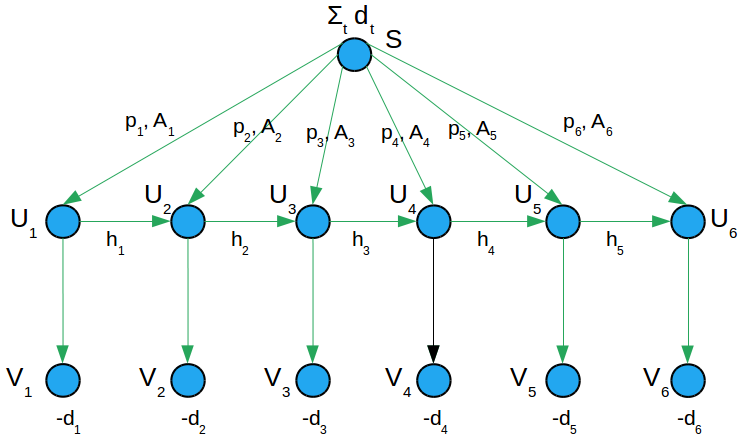
\includegraphics[height=8.5cm]{images/graph3.png}
	\label{fig:WagnerWhitin}
\end{figure}

\subsubsection{Proprietà della soluzione ottima}
\textbf{Teorema.} In una soluzione ottima non può mai avvenire che la domanda del periodo $t$ venga soddisfatta sia dalla produzione che dal magazzino, ovvero:
\begin{center}
	$I_{t-1}\cdot x_{t}=0;\;t=1,...,T$
\end{center}
\begin{figure}[H]
	\caption{}
	\centering
	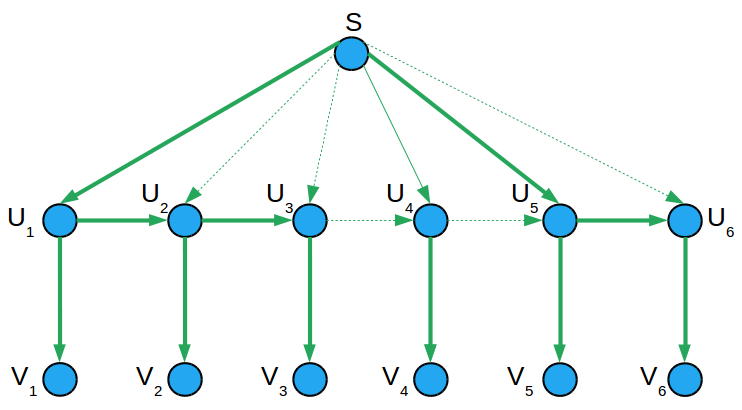
\includegraphics[height=5.6cm]{images/graph4.png}
	\label{fig:PossibileSoluzione}
\end{figure}

\subsubsection{Algoritmo di soluzione (di complessità $O(T^{2})$)}
Si costruisca un grafo aciclico di $T+1$ vertici.\newline
Si definiscano gli archi $j,k)$ per $j=0,...,T-1$ e $k=j+1,...,T$.

L'arco $(j,k)$ rappresenta la decisione di produrre all'inizio del periodo $j+1$ quanto serve per soddisfare le domanda complessiva dei periodo $j+1,\;j+2,...,k$.

Il costo $M_{jk}$ dell'arco (j,k) è pari al costo per produrre nel periodo j+1 la quantità $\sum_{r=j+1}^{k}d_{r}$ più i costi di stoccaggio:
\begin{center}
	$M_{jk}=A_{j+1}+p_{j+1}\displaystyle\sum_{r=j+1}^{k}d_{r}+\sum_{t=j+1}^{k-1}h_{t}(\sum_{r=t+1}^{k}d_{r})$
\end{center}
\begin{figure}[H]
	\caption{}
	\centering
	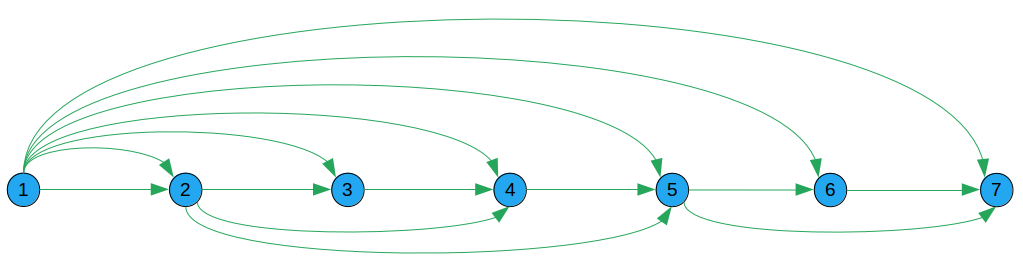
\includegraphics[height=4.2cm]{images/graph5.png}
	\label{fig:PossibileSoluzione2}
\end{figure}

Ogni soluzione del modello di Wagner-Whitin corrisponde ad un cammino da $0$ a $t$ in questo grafo aciclico.\newline
Il cammino di costo minimo fornisce la soluzione ottima.